\chapter{Network Topology}
In order to test the aforementioned algorithms, it is necessary to build  and evaluate a topology that represent an SG network. The algorithms work with data, their function is to gather and collect it  and compute aggregation functions in a distributed way. Therefore, our focus to build a testing network is the SG information subsystem. As it was stated in the chapter\ref{chap:sg}, the AMI system is part of the information subsystem where meter information, the one we are interested in, is  treated. So, our topology must represent an AMI Network, with the smart meter data used to compute the aggregation function. We are interested in the collection part of that data and the process made to update the prices accordingly to production/consumption of the network. In the following section, we will characterize more precisely what scenario we assume and which communication assumptions we make.


\section{Communication}
When building a topology or a network, is important to know and consider  the communication technology used and what are the assessments we make. In AMI networks, there are many options, both wired and wireless, for as many needs. A suitable choice for a Smart Meter data collector could not be a suitable choice for a central facility substation flow because of the different needs and requirements. Since in this work focused in the data collected by the aggregators and the communication between s, the choice of a communication infrastructure must be among the technologies used in the Low Voltage grid, i.e., where the metering is performed. Therefor, wee assume an AMI network that uses a PowerLine Communication Infrastructure, used, for example, in EDP InovGrid\cite{matos2013inovgrid} and Iberdrola pilot projects \cite{sendin2012performance}
\subsection{PowerLine Communication}
PowerLine Communication(PLC) is a communication technology which uses the installed electrical cables to transmit data. It has been the first choice for communication with the electricity meter due to the direct connection with the meter and successful implementation of AMI in urban areas where other solutions struggle to meet the need of utilities\cite{gungor2011smart}. \\
The typical application of the PLC is to connect the smart meter to the data concentrator. The SM communicates the consumption or production data to the collecting device through the power line. After the collection from the meters, normally, the data aggregator send the  stored data to a central facility, that is owned in most cases by the electrical company,  through a more fast technology like optic fiber. In Europe the majority of the transformers serves 200 customers or more, so the data collectors are located in the LV side, in the transformers and using PLC to communicate with the meters. In the USA, the concentrator or aggregator is often in the MV side of the grid, due to the low number of end points per transformer. The large number of end-points per transformer in Europe does not require to locate the concentrator up in the substation or on the MV side, so it can be conveniently located on the LV section of the grid. REMPLI project tells us that unlike solution based on ZigBee os Wifi, PLC-based AMI have a proven track record of being able to avoid network congestion when cooperative schemes are employed\cite{galli2011grid} \\
As it was stated before, one of mains advantages of using a PLC based communication infrastructure is the cost to deploy.  The fact that the cables are already installed makes PLC a more appealing technology compared to other wired solutions. Considering only the costs, PLC can even compare to the wireless proposed solutions\cite{gungor2011smart}. \\
The standardization efforts on PLC networks, the cost effective, ubiquitous nature and widely available infrastructure can be the reason for its strength and popularity. It is also well suited for urban areas for smart grid applications, besides AMI  application like metering, PLC can also be used to monitoring and control because, once again, the involved areas are already covered.\\
Although it popularity, PLC still represents some disadvantages mainly because of the nature of the channel and because of some technical problems. The communication channel is a harsh and noisy environment that makes it difficult modeled. Furthermore the network topology, the number and type of the devices connected to the power lines, wiring distance between transmitter and receiver, all, affect the quality of signal that is transmitted over the power lines. However, recent modulation techniques and technologies are overwhelming the mentioned difficulties, mitigating the noisy environment by reducing the data rates and the bandwidth.\\ 



\section{Data Collector/Aggregator}
Data collectors or data Aggregators are devices installed in the Low Voltage side of the Grid, in the European case, or in the Medium Voltage side of the grid in the American case, because the ratio SM per transformer it lower in USA than in Europe. They normally serve as data storage where a set of SMs are directly connected to it sending the consumption or production of a household.\\
Data Collectors normally serve as a storage but this is not a rule that apply to all, there are cases where the data aggregators perform more operations. In the PowerMatching City project case, the data collectors receive data in bid format, to buy or to sell and then calculate the price of the energy to  others buy and sell. They work in market way, not only collecting information, but also making decisions about prices. In the case of InovGrid, the data collectors just collect data. Other projects lack the existence of this devices, using instead a cloud based service, others use it inside the house to collect data from different electrical devices to know which ones are consuming the most. As it was presented in chapter \ref{chap:sg},  SG projects which don't require the use of any data collector propose a architecture that enable the smart meters to directly send their data to a data center through a cloud based service. These different architecture exist because there are different goals in the different pilot projects. The ones which use big data to perform detailed statistical report to raise awareness in the costumers require the maximum amount of data as possible. In the cases where the goal is achieve a ideal strategy to buy/sell energy, provide a reasonable Demand Side Management and useful information to the operation side don't require a big amount of data, so they use an mid level set of devices to aggregate the data.\todo{Review this idea} \\

\section{Demand Side Management and Real Time Pricing}
Demand Side Management refers to a serie of strategies and policies to load balance the demand efficiently in order to prevent very high demand peak hours, preventing the overload of the production and the occurrence of blackouts or faults. Although applied in the SG and AMI scenario, it is not a recent trend, demand side management has been considered since the early 80's \cite{samadi2010optimal}.\\
One of the application of Demand Side Management in the Low-Voltage Grid it Demand Response(DR) which refers to the ability to make demand able to respond to the varying supply of generation that cannot be scheduled deterministically. DR is  a means to alleviate peak demand and also to bring more awareness on energy usage to the consumer. It is believed that DR will allow a better control of peak power conditions, maximize the use of available power and increase power system efficiency.\\
A more specific example of how DR can be applied is by real time pricing which is one of the strategies to achieve and realize Demand Side Management. Real time pricing is a pricing policy, basically it consist of upgrading the prices accordingly to the demand and the supply, in other words, the prices vary as the demand increases or decreases along periods of time. This policy tend to persuade the costumer to reduce their energy consumption during the peak hours, since the price is higher, and increase slightly outside the peak hour, when the price is lower.\\
In \cite{taqqali2010smart} is realized a research regarding the aforementioned policies in UAE. The experience states that costumers react better to peak time adaptive tariff. Also, it is stated that with these pricing policies, costumers are more aware of their consumption and, for consequence, more willing to reduce their consumption during peak hours. The authors also point that consumption demand is reduced during the peak hour while balancing it.\\
 \cite{lin2014designing} proposes an optimal pricing policy for aggregators. The aggregator "buys" the electrical energy from the supplier, and regarding the necessary demand, defines the price. The time is spited in $K$ time intervals, in the $k$ interval the aggregator must make decisions based on the $k-1$ interval information about demand and energy available from the electrical company. The goal is to maximize the profit, but it can also be applied to reduce the demand during peak hours if the decisions are made for reducing the demand when the supply is low and the demand high. The behavior is similar to the PowerMatching city, but the aggregator have instead information about bids to buy or sell energy. \\
We assume a real time pricing scenario, where each aggregator should have a behavior similar to \cite{lin2014designing} and the PowerMatching city, i. e., the aggregator make decisions regarding the energy price based on the supply from the electrical company, on the total consumption from the costumers and  also from their production by renewal energy sources. The pricing policy followed is outside the scope of this work, we only consider the problem of a given time, evaluate the overall consumption or production, so the aggregators can make the pricing decision accordingly.\\ 

\section{Case Study}
In this work we do consider the existence of data collectors. We don't make any assumption regarding the number of households connected per data collector. Instead we assume that a certain number of smart meters are connect to a data collector, therefore, the device contains information regarding the connected houses consumption and production. 
\begin{definition}
For a data collector $D$, a set $H$ of households with a smart meter are connect to it. $H$ is defined as
\begin{equation*}
H = \{ h_1,h_2,h_3, \dots , h_n \}
\end{equation*}
Where $n$ is the size of $H$ and $n >= 1$
\end{definition}

\begin{definition}
At a given time $k$, a data collector $D_k$ contains a consumption $C_{D_k}$ where is defined:
\begin{equation*}
C_{D_k} =  \sum_{i=1}^{n} c_{i}
\end{equation*}
where $n$ is the size of the set $H$ and $c_{i}$ is the consumption of the $i$ household connected to the data collector $D_k$ at time $k$
\end{definition}
 Also, we assume that each data collector is located not only on the MV/LV transformer, but in every substation of the network which contains electric equipments (e.g., rails, bus bars, electrical switches, etc). Although we don't cover the security aspects of the data collectors, not only information security,privacy and integrity, but also physical information, there are in the current projects security measures to avoid the violation/steal of the data collector and encryption techniques and ciphers are also applied to provide security information guarantees. Once again, security issues are not cover in this work. \\
In the InovGrid case \cite{matos2013inovgrid} and in Iberdrola projects \cite{sendin2012performance}, the data collectors only communicate the data to the electrical company, and not among each other. We took the example of the PowerMatching city, and other proposed SG architecture seen in \ref{chap:sg}, and consider not a hierarchical network composed by households, data collector substations, and the data center as a sink, but a network of data collectors that communicate with each other.Although they communicate the overall network consumption/production with the electrical company, they share their data in order to all the collectors in order to compute an aggregation function without the need of a central device.\\
To complete our scenario, we assume one more similar aspect to the PowerMatching city, but, instead of the data collector receive the data in a bid format to buy or sell energy, we consider consumption and production values. Therefore, the price of the energy should be calculate according to this 2 variables, as in a PowerMatching market. We will not cover the market aspect, the problem we focus on it knowing the consumption or production of a data collector network using Distributed Aggregation Algorithms.\\
\subsection{Network Architecture}\label{sec:arch}
This work focus on the Low Voltage power grid network, with voltage $V_{LV} <= 10 kV$, and evaluate a Smart Grid scenario. We start by choosing a Low Voltage power grid network sample and define a Smart Grid graph. For the low voltage power grid sample graph, we choose one from the work of \cite{pagani2013grid} and define a Smart Grid graph.
\begin{definition} 
A Smart Grid graph is a graph $G(V,E)$ such that each element $v_i \in V$ is either a substation with electrical equipment or a transformer os a physical power grid with a data collector installed, There is a edge $e_i,j =(v_i,v_j) \in E$ between two nodes if there is physical cable  that enables a PowerLine communication connecting directly the element represented by $v_i$ and $vj$ 
\end{definition}
With the definition of our Smart Grid graph, we need to bring and specify some important properties into the graph definition.
Each edge $e_i,j\in E$ represent a physical cable, enabling a PowerLine Communication between the data collectors. Our Smart Grid graph is a weighted graph, we consider channel capacity in bps a suitable weight for the edges. We calculate the capacity of the channel by the channel capacity function defined in \cite{biagi2010location} , assuming that all channel are Gaussian Channels. We also assume that the communication uses the CENELEC A band.
\begin{definition} Channel Capacity is defined by the function $M_{ij}$
\begin{equation*} 
M_{ij} = \int\limits_{B_1}^{B_2}  C  \left( \frac{S_T | H_{ij}(f) |^2} {N_0\Gamma} \right)  \mathrm{d}f
 \end{equation*}
Where $H_{ij}(f)$ represent the transfer function between nodes $v_i$ and $v_j$, $\Gamma$ is a gap factor to account for practical coding schemes, $B_1 = 9kHz$ and $B_2 = 95 kHz$ are the lower and upper frequency of the CENELEC A band, $S_T$ represent the power spectral density, $N_0$ is the background noise modeled as white Gaussian noise and $C(\gamma)$ is the capacity at signal-to-noise power ratio (SNR) of $\gamma$
\end{definition}
We assume the same reference values in \cite{biagi2010location}, $S_T=-60dBV^2/Hz$, $N_0=-138 dBV^2/Hz$ and $\Gamma = 10$. $C(\gamma)$ is defined as:
\begin{equation*}
C(\gamma) = \log_2(1+\gamma)
\end{equation*}
We assume that all the cables are of the type NAYY150SE, the cable lengths are the ones  provided the samples used in \cite{pagani2013grid} and the other physical characteristics are taken from \cite{lampe2011cooperative}.\\
The figure \ref{fig:network} represent illustrate the graph represent the network used for the tests.
\begin{figure}[h]
\centering
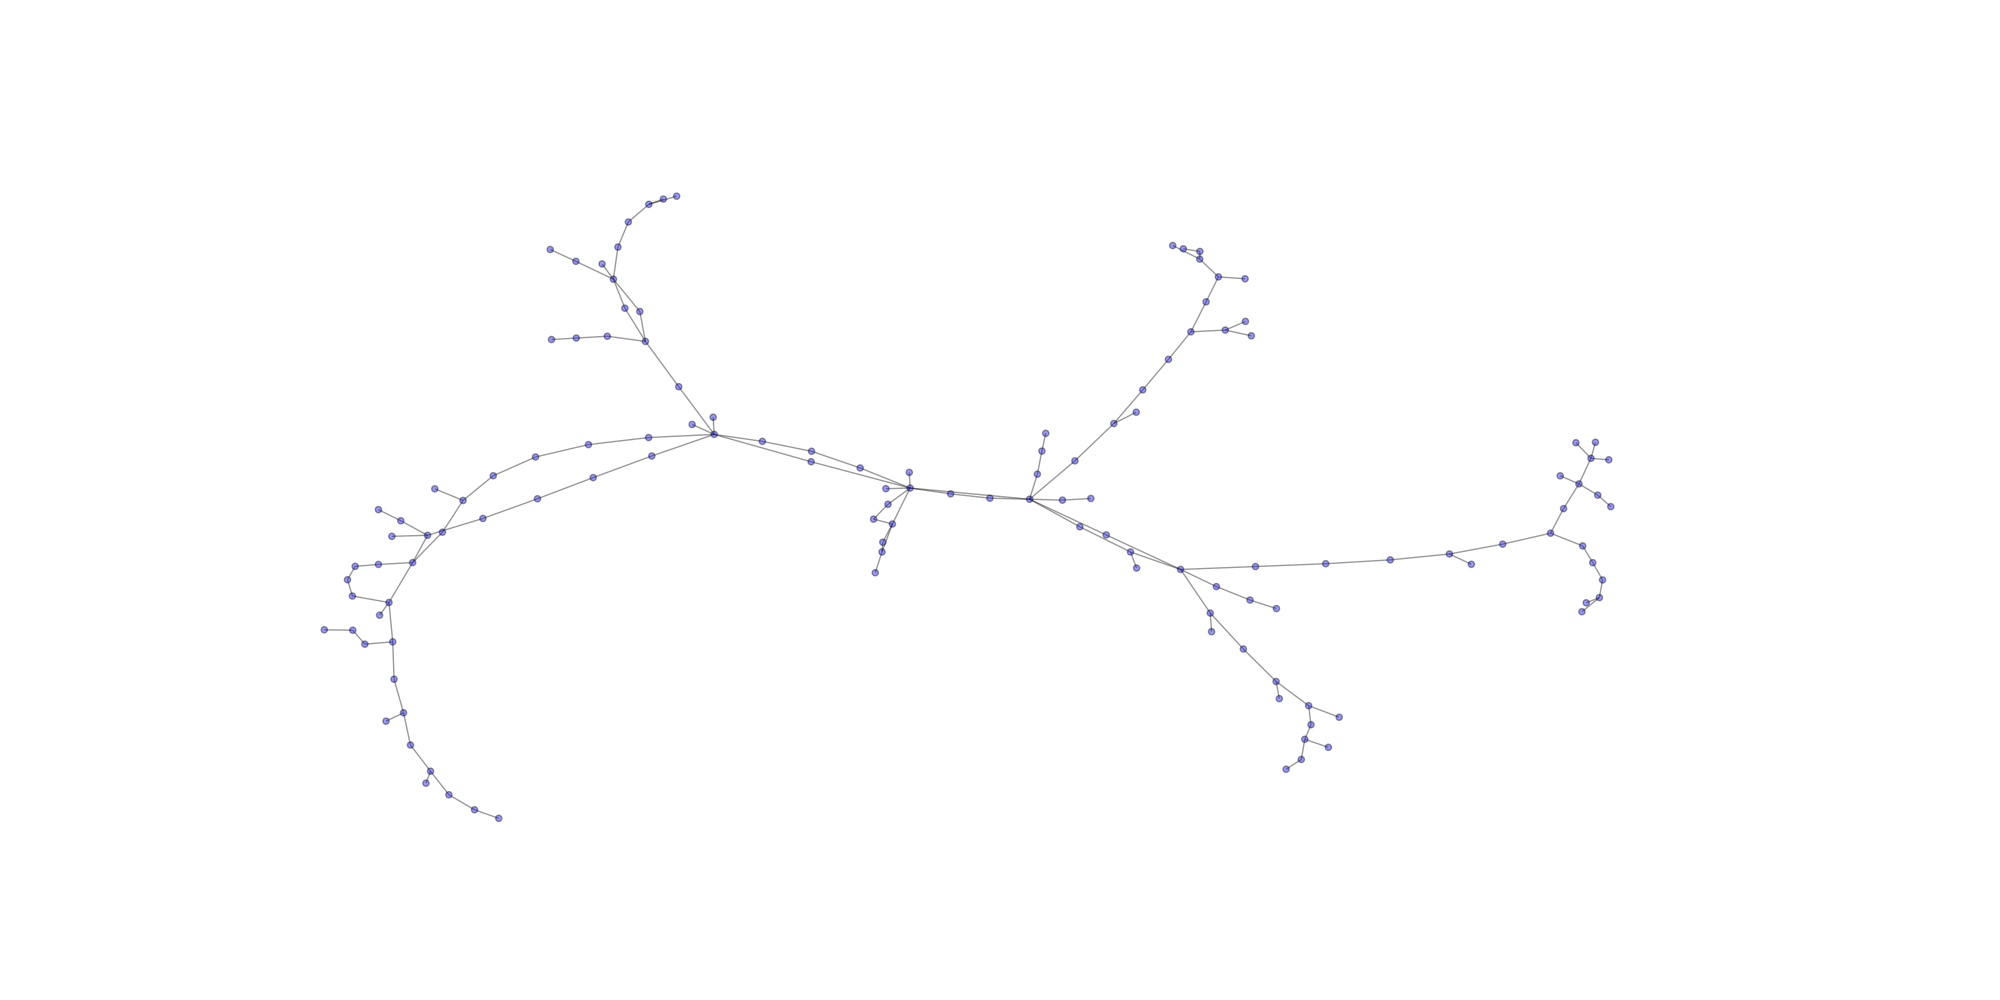
\includegraphics[width=1\textwidth]{/Users/rafaelremondes/UM/MEI/Thesis/DistributedAggregationAlgortihmsSM/Writing/Images/network}
\caption{\label{fig:network}  Smart Grid Graph}
\end{figure}

\section{Used Aggregation Algorithms}
In this section is presented the aggregation algorithms used. In Chapter \ref{chap:dda}  there is only  a brief description of all the Algorithms, here we formalize the algorithms used. The problem the algorithms need to solve is a evaluate the consumption of all the data collectors, so the algorithms tested are the ones who allow us to do so. We choose the \textit{Averaging} algorithms and based on \textit{Sketches} because they are designed to evaluate the function \textit{AVERAGE}, and most important, the function \textit{SUM}. Other algorithms are more suitable to understand a distribution of values in a network or to evaluate  its size.\\
\subsection{Push-Sum}
\begin{algorithm}
\caption{Push-Sum Algorithm}
\begin{algorithmic}[1]
\STATE Let $\{ (s_r,w_r)\}$ be all pairs sent to $i$ in round $t-1$
\STATE Let $s_{t,i} :=  \sum_{r} s_r$ , $w_{t,i} := \sum_{r} w_r$
\STATE Choose a target $f_t(i)$ uniformly at random
\STATE Send the pair $ \left(  \frac{1}{2} s_{t,i} ,  \frac{1}{2} s_{t,i}  \right) $ to $f(i)$ and $i$ (yourself)
\STATE $\frac{s_{t,i}}{w_{t,i}}$ is the estimate of the average in step $t$
\end{algorithmic}
\end{algorithm}
In the Push-Sum algorithm \cite{kempe2003gossip}, initially, each node generates a pair $(s,w)$ where $s$ is its value to aggregate and $w$ its weight, initiated to one. At every round $t$, each node $i$ evaluate $s_r$ and $w_r$ which are the $SUM$ of all the pairs $(s,w$ send to $i$ in the previous round. After evaluating $(s_r,w_r)$, send half the $\frac{1}{2}s_r$ and  $\frac{1}{2}w_r$ to a randomly choosed neighbor and to itself. The $AVERAGE$ in the round $t$ is the $SUM$ of all received $s$ in the round $i$ plus $s_r$ divided to the e $SUM$ of all received $w$ in the same round $i$ plus $w_r$. To evaluate the total $SUM$ of the values instead of the $AVERGE$, the algorithm suffers one slightly difference. Every node starts with initial weight equal to 0, except for one node, which its initial weight is 1.
\subsection{Flow Updating}
\begin{algorithm}
\caption{Flow Updating}
\begin{algorithmic}
\STATE \textbf{State Variables:}
\STATE $f_{ij}, \forall j \in D_i $, flow, initially $f_ij = 0$
\STATE $e_{ij}, \forall j \in D_i$, estimates, initially $e_{ij} = 0$
\STATE $v_{i}$, input value
\\
\STATE \textbf{message-generation function:}
\STATE msg$(i,j) = (f_{ij},e_{ij}),\forall{j}\in D_i$
\\
\STATE \textbf{state-transition function:}
\FORALL {$(f_{ji},e_{ji})$ \textbf{received}}
\STATE $f_{ij \leftarrow -f_{ji}}$
\STATE $e_{ij} \leftarrow e_{ji}$
\ENDFOR
\STATE $e_i \leftarrow \frac{\left(v_i - \sum{j \in D_i} f_{ij}\right)+\sum{j \in D_i} e_{ij}}{|D_i|+1}$
\FORALL {$j \in D_i$}
\STATE $f_{ij} \leftarrow f_{ij} + (e_i-e_{ij})$
\STATE $e_{ij} \leftarrow e_i$
\ENDFOR
\end{algorithmic}
\end{algorithm}
\todo{Alinhar isto}
In Flow Updating\cite{jesus2009fault}, each node $i$ initializes its state variables, a set of pair $(f_{ij},e_{ij})$ where $f_{ij} = 0$ and $e_{ij} = 0$, a pair correspondent to each neighbor, contain the flow and an estimate. Also, the node holds an input value $v_i$, the value to aggregate. \\
At every round, a node generates an send a message to each neighbor $j$, the node $i$ send its correspondent flow and estimate $(f_{ji},e{ij})$.\\
The next step, the state transition function, each node starts by updating the local flows and estimates with the corespondent received one from the corespondent neighbor. Thereafter, each computes a new prediction of the aggregation value $e_i$ by averaging the received estimates and the one locally calculated by the equation bellow, that evaluates the overall estimate $AVERAGE$ of the network. It updates after its state accordingly: the new estimates equals to the one previous estimate calculated and the flow $f_{ij}$ is added the difference between the new estimate $e_i$ and the received estimate from$j$.
\todo{difference to calculate the SUM}
\begin{equation*}
a_i = v_i - \sum{j \in D_i} f_{ij}
\end{equation*}
\subsection{PushPull}
\begin{algorithm}
\caption{Push-Pull Active Thread}
\begin{algorithmic}
\STATE $q$ $\leftarrow$ $getneighbour()$
\STATE send $s_p$ to $q$
\STATE $s_q \leftarrow$ $receive(q)$
\STATE $s_p \leftarrow$ $update(s_p,s_q$)
\end{algorithmic}
\end{algorithm}
\begin{algorithm}
\caption{Push-Pull Passive Thread}
\begin{algorithmic}
\STATE $s_q \leftarrow receive(*)$
\STATE send $s_p$ to $sender(s_q)$
\STATE $s_p \leftarrow update(s_p,s_q)$
\end{algorithmic}
\end{algorithm}
In Push-Pull protocol \cite{jelasity2005gossip}, the nodes work with two \textit{threads}. The active \textit{thread} runs once at each round. Selects a neighbor $q$ at random and send to it its value to aggregate $s_p$, afterwards, expects to receive the value $s_q$ from the neighbor $q$. Update them the value $s_p$ by averaging $s_p$ and $s_q$.\\
Each node runs the passive \textit{thread} in background, all the time. This background process basically sends the hold value $s_p$ to every requested neighbor $q$. After sending it, the node updates it value $s_p$ the same way as the active \textit{thread}.\\
To calculate the $SUM$, instead of the $AVERAGE$, a pair is exchanged instead of only a value to average. One of the value is the value to average an the other value of the pair is the value to calculate the size. The overall $SUM$ will evaluated by multiplying the size to the average. Note that to evaluate the size, every node should start the value to calculate the size as 0, except for one node that initializes with 1, the same principle as in Flow Updating and Push-Sum.
\subsection{Extrema Propagation}
\begin{algorithm}
\caption{Extrema Propagation}
\begin{algorithmic}
\STATE \textbf{const} $K$
\STATE \textbf{var} $n,x[1..K]$
\REQUIRE Init
\STATE $n \leftarrow neighbours(self)$
\FORALL{$l \in 1..K $}
\STATE $x[i] \leftarrow rExp(1)$
\ENDFOR
\STATE Send $x$ to every p $p \in n$
\REQUIRE Receive $m_1..m_j$ from all $p \in n$
\FORALL{$l \in 1..j$}
\STATE $x \leftarrow pointwisemin(x,m_l)$
\ENDFOR
\STATE Send $x$ to every $p \in n$ 
\REQUIRE Query
\RETURN $\hat{N}$
\end{algorithmic}
\end{algorithm}
Extrema Propagation \cite{baquero2012extrema} is based on \textit{sketchs}, each node holds and shares a \textit{sketch}, an auxiliary data structure to calculate the desired aggregation function. Each node holds an array $x$ with dimension $K$, and initializes every $x_i \in [1..K]$ equal to a random value calculated by the function $rExp(1)$, which returns a random number with and exponential distribution of rate parameter 1. $n$ is initialized as the set of all neighbors to a node $i$, thereafter, the each node send the array $x$ to every neighbor from $n$. At each round, every single node from each message $l$ from $m1..m_j$ updates the array $x$ begin equal to the $pointwisemin(x,m_l)$. After updating $x$, send the updated  array to each neighbor from $n$.\\
To calculate the estimate of the size of the network $\hat{N}$ in each round, each node computes the equation:
\begin{equation*}
\hat{N} = \frac{K}{\sum{i=1}^{K} x[i]}
\end{equation*}
To calculate the $SUM$ instead of the size of the network, the $rExp()$ function takes as argument the value to aggregate instead of 1.
\subsection{RIA LC/DC}
RIA LC/DC \cite{fan2010efficient} is also based on \textit{sketchs}. Each node initially holds a \textit{sketch}, an array of zeros of size $m$. Each node initializes the array by mapping, using a random function that gives the index of the array, the value to aggregate into the sketch, bit by bit. For example, if the value to aggregate is 3, the node should map the values 1, 2 and 3. After initialized the sketch, at each round the nodes share with their neighbor the sketch and merging the received ones with the sketch hold locally by using \textit{XOR}. In order to calculate the estimate $\hat{n}$ of the SUM is calculated by
\begin{equation*}
\hat{n} = -m*ln(V_n)
\end{equation*}
Where $V_n$ is equal to the division of the number of zeros in the \textit{sketch} and the size of $m$.
